\subsection{Real-time Performance Evaluation}
% Right arrow in LaTeX: $\rightarrow$ or \to

Since the development of the project is currently underway, the mixer has not been developed yet,
which is essential for getting all the components working together for stress test. In the meantime, 
the callback execution times for each components are measured using the RAII timer (Appendix) outside 
the audio engine, and a buffer size of 512 floats, and a sample rate $f_s = $ \SI{44100}{\hertz}. 

The buffer latency is,
$$\frac{512}{44100} \approx 11.61\, ms$$

Multiple measurements of the execution time are taken using the timer code in \Cref{app:exec_time}, Listing \ref{lst:raii-timer}, 
and the statistical results for each of the components are tabulated in \Cref{tab:audio_component_benchmark}.
% TODO: Add the code for the timer

\subsubsection{Measurement Results}

\begin{table}[htbp]
    \centering
    \caption{Processing Time Measurements of Audio Components}
    \label{tab:audio_component_benchmark}
    \begin{tabular}{lrrr}
        \toprule
        \textbf{Component} & 
        \textbf{Mean ($\mu$s)} & 
        \textbf{Max ($\mu$s)} & 
        \textbf{Std. Dev. ($\mu$s)} \\
        \midrule
        WAV Audio Streaming & 24.274 & 52.380 & 3.140 \\
        Fluidsynth Rendering & 36.882 & 80.725 & 6.763 \\
        Osc-based Synthesizer & 57.318 & 126.401 & 18.355 \\
        SFZ Rendering & 19.752 & 47.370 & 4.005 \\
        RBJ Biquad Processing & 13.761 & 60.452 & 3.540 \\
        RBJ Biquad Parameter Change & 50.243 & 121.524 & 20.831 \\
        SVF Filter Sweeping & 41.585 & 180.045 & 14.300 \\
        Reverb & 810.875 & 1580.370 & 106.859 \\
        Compressor & 28.728 & 86.100 & 12.551 \\
        Echo/Delay & 7.795 & 30.291 & 4.884 \\
        \bottomrule
    \end{tabular}
\end{table}

It is observed that reverb has the worst callback times of all, which is expected, because of the heavy
computation led by randomization, multi-channel processing, diffusion, etc. And the echo/delay effect has
the lowest callback time. Which means, reverb cannot be assigned to each of the components individually, but
rather share a single reverberation system with multiple tracks.

Also, the standard deviation seems to be positively correlated with the callback 
execution time, since larger callback times have greater deviation time. Since these deviation times are
small compared to their respective mean callback times, it can be assumed that the audio engine is less
prone to jitter with these components.

While comparing the callback times between the RBJ Biquad parameter change, and the SVF Filter sweeping,
the total mean execution time and worst-case execution time are calculated to be \SI{64.004}{\micro\second} and 
\SI{181.976}{\micro\second} respectively, which are larger compared to the SVF counterparts. This supports
the decision about using SVF for frequency sweeping in synthesizer, as opposed to Biquad coefficient calculation.

And finally, it is also expected to have the Oscillator-based synthesizer to have higher execution time, compared
to Fluidsynth and SFZ counterparts, because the inexpensive ones solely rely on recorded wavetables. It is also expected
to achieve heavier computational workload when more synth-related DSP components are added, because currently the synthesizer
is currently in the rudimentary stage with unison effect only.

\subsubsection{Final Verdict}
To calculate the overall execution time, a mockup of an innocuous electronic/trance project is created only by assigning instruments 
with their appropriate audio effects, ignoring any audio designing or composing music (\Cref{prompt:mockup_session}) \cite{openai_chatgpt}. 
As discussed in the Introduction section, each thread can contain multiple tracks, 
so that these tracks can be mixed in parallel which can reduce the overall execution. Please refer to the flow diagram in 
\Cref{fig:daw_mockup}.

\begin{figure}[ht]
  \centering
  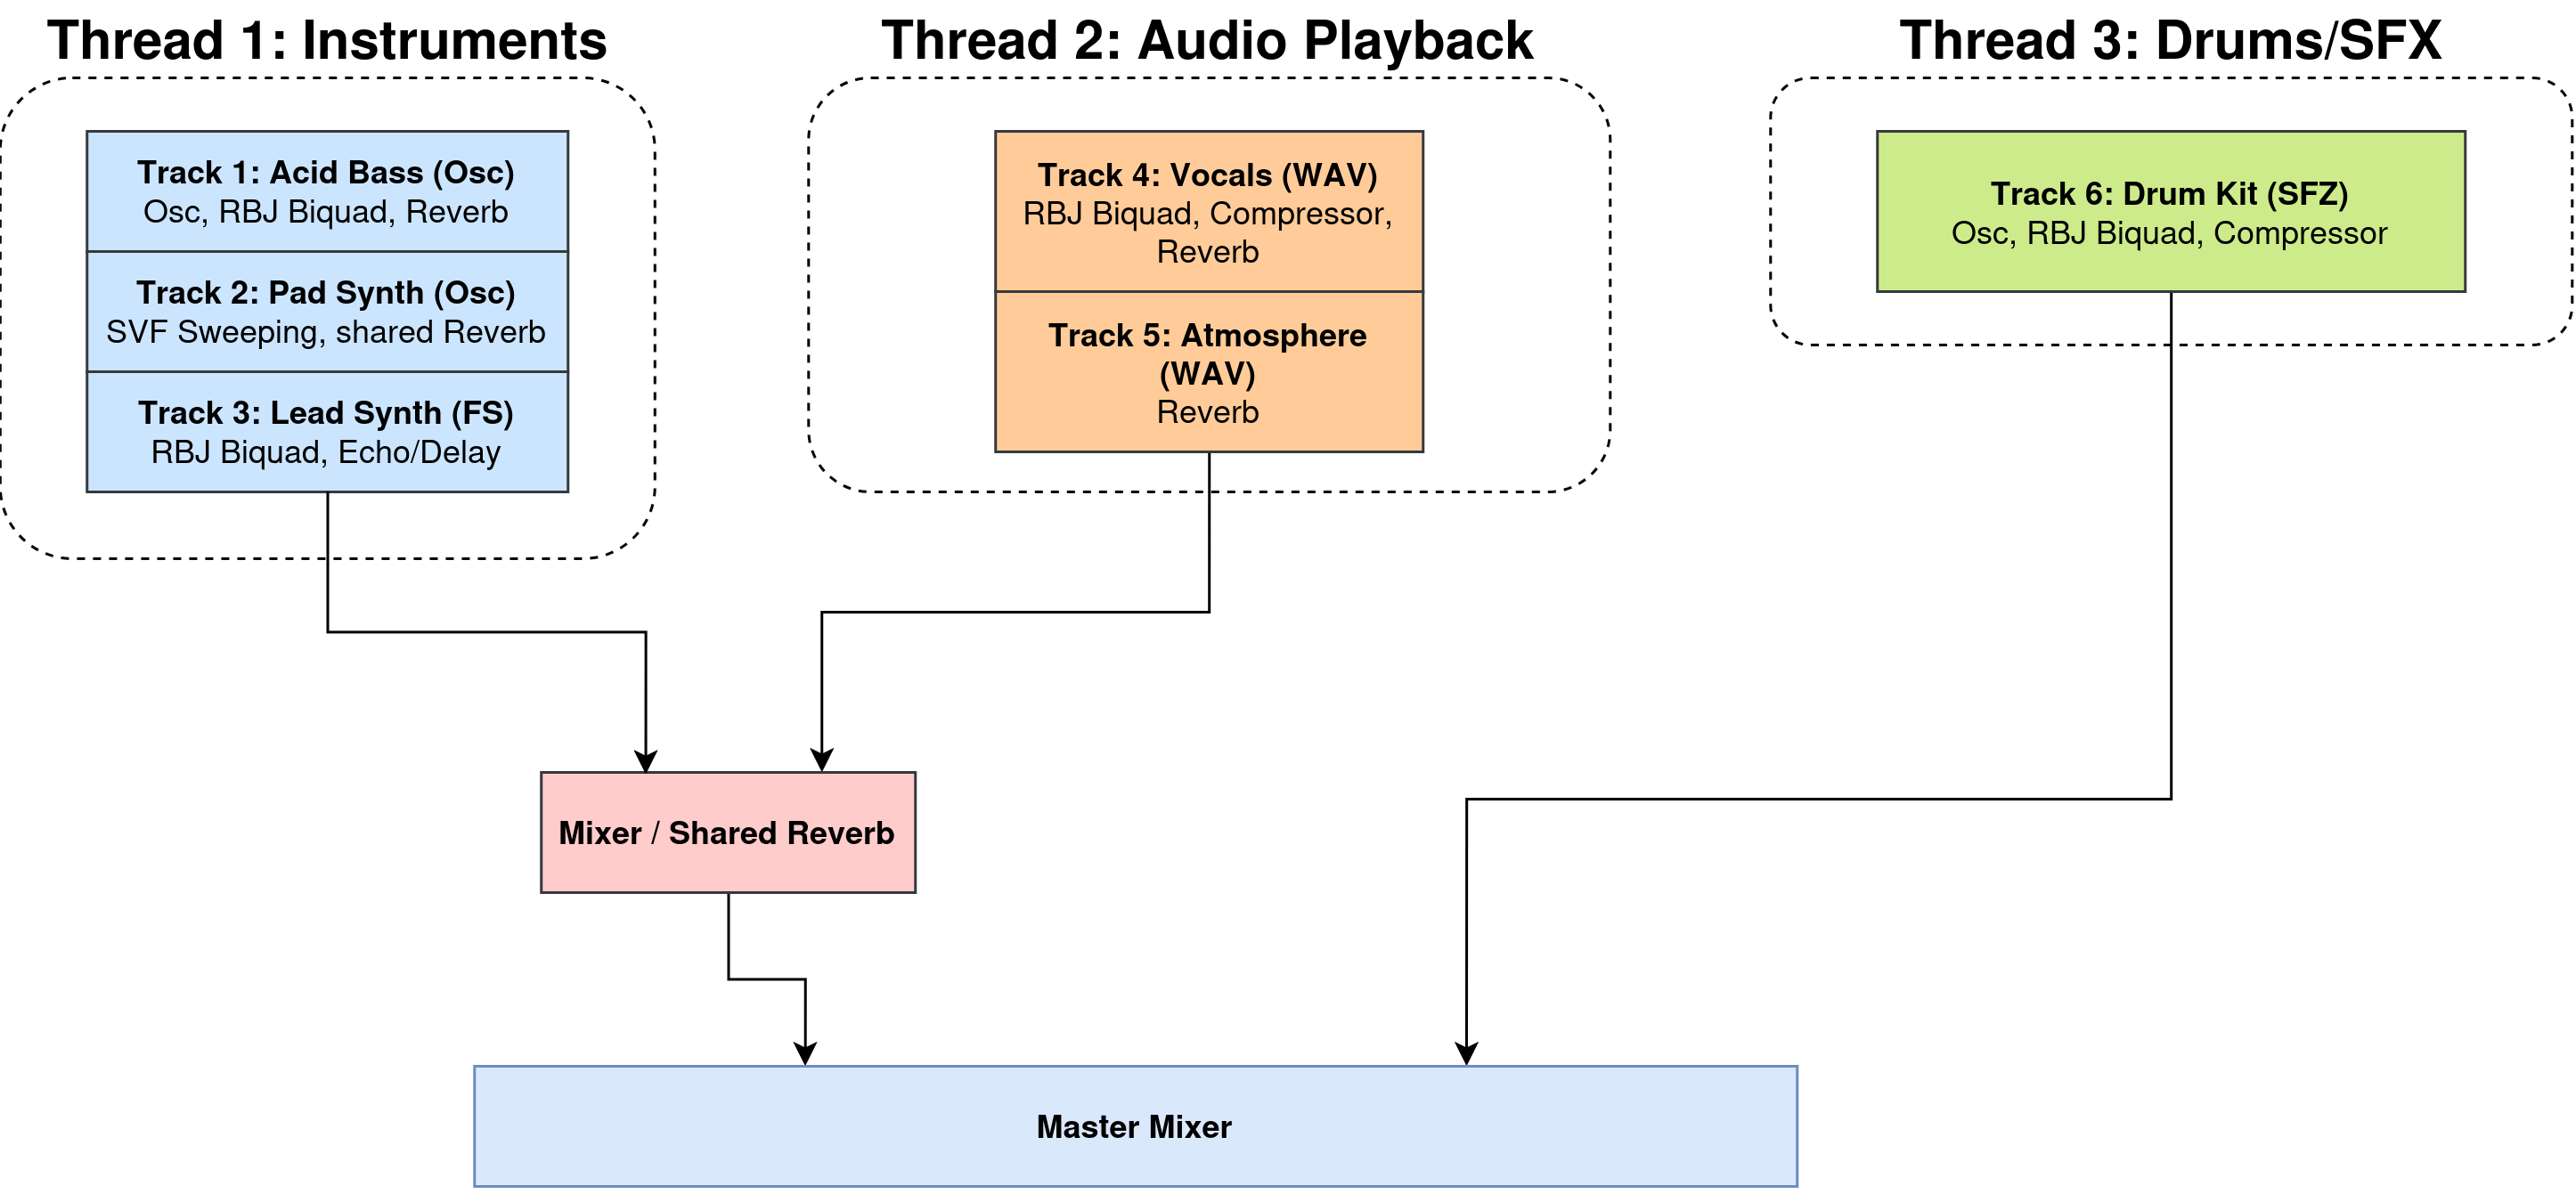
\includegraphics[width=\linewidth]{discussion/benchmark/figures/DAWMockup.png}
  \caption{Arbitrary Example of a DAW Session Showing the Arrangement of Tracks}
  \label{fig:daw_mockup}
\end{figure}

Assuming that the workloads from the mixers, and the audio engine callback times are negligible,
the following list shows some calculations for each of the tracks, including master audio effects using the mean
execution times, ignoring any reverbs at that stage:

\pagebreak

\begin{enumerate}
    \item \textbf{Thread 1}:

        \subitem Track 1 (Acid Bass) $\rightarrow t_{T1} = 57.318 + 13.761 = 71.080\,\mu s$
        \subitem Track 2 (Pad Synth) $\rightarrow t_{T2} = 57.318 + 41.585 = 98.904\,\mu s$
        \subitem Track 3 (Lead Synth) $\rightarrow t_{T3} = 36.882 + 13.761 + 7.795 = 58.439\,\mu s$
        \subitem \textbf{Total}: $t_\text{th1} = 228.422\,\mu s$

    \item \textbf{Thread 2}:
        \subitem Track 4 (Vocals) $\rightarrow t_{T4} = 24.274 + 28.728 + 7.795 = 60.797\,\mu s$
        \subitem Track 5 (Pad Synth) $\rightarrow t_{T5} = 24.274\,\mu s$
        \subitem \textbf{Total}: $t_\text{th2} = 85.071\,\mu s$
    
    \item \textbf{Thread 3}:
        \subitem Track 6 (Lead Synth) $\rightarrow t_{T6} = 19.752 + 13.761 + 28.728 = 62.242\,\mu s$
        \subitem \textbf{Total}: $t_\text{th3} = 62.242\,\mu s$
        
\end{enumerate}

Thread 1 takes the longest amount of time to run compared to other threads, so the other utilities, including
the reverb mixer and the master mixer has to wait for at least \SI{228.42}{\micro\second}. Then, the reverb
has to process the audio for about \SI{810.875}{\micro\second}. Therefore, the overall mean execution
time would be,

$$
\bar{t} = 228.42 + 810.875 = 1039.295\,\mu s = 1.039\, \text{ms}\, (< 11.6 \text{ms})
$$

Which means that the audio engine will work smoothly without any interruptions or artifacts. However,
the calculations using the worst-case execution times are already conducted using the same principle as above.
Therefore, the worst-case execution time is estimated to be \SI{2245.13}{\micro\second}, and will still meet 
the buffer deadline.

Therefore, these estimations provide evidence that the DAW engine has the potential to survive that amount of workload. But the scalability
can further be extended by adding more tracks to perform the actual stress test, i.e. getting everything to work together inside the audio engine 
in real time using more than 6 tracks with audio effects. Moreover, the evaluated workload does not require multithreading to meet real-time constraints,
based on these estimation. However, parallel processing may become beneficial as additional workload-heavy instruments, effects, or plugins are introduced.
